Magnetic materials can be found across a wide range of modern technologically important applications, such as data storage and spintronic devices,\cite{zutic2004spintronics} quantum computing,\cite{de2021materials} energy conversions,\cite{kitanovski2020energy} and sensors.\cite{gloag2019advances}  Fundamentally, the ground-state magnetic structures of materials play a deterministic role in how the materials may be applied in functional magnetic devices, thus determining the magnetic ground states of solids, and how the interactions amongst spins, electrons and orbitals stabilise these magnetic states, are the key goal for applying electronic structure theory, particularly DFT, to study the magnetic properties of materials. From the perspective of energy landscape, this introduces additional degrees of freedom in the PES $E(\{\bm{R}_i\})\to E(\{\bm{R}_i\},\{\bm{s}_i\})$, in which now the energy of the atomic structure is not only dependent upon its ionic positions $\{\bm{R}_i\}$, but also the corresponding configurations of the net electron spin on the individual ion $\{\bm{s}_i\}$ in the structure. This implies that, for a fixed set of $\{\bm{R}_i\}$,  we will also need to sample different spin configurations $\{\bm{s}_i\}$, in account for this extra degree of freedom, to determine the magnetic ground state of a given material.

\begin{figure}[tb]
    \centering
    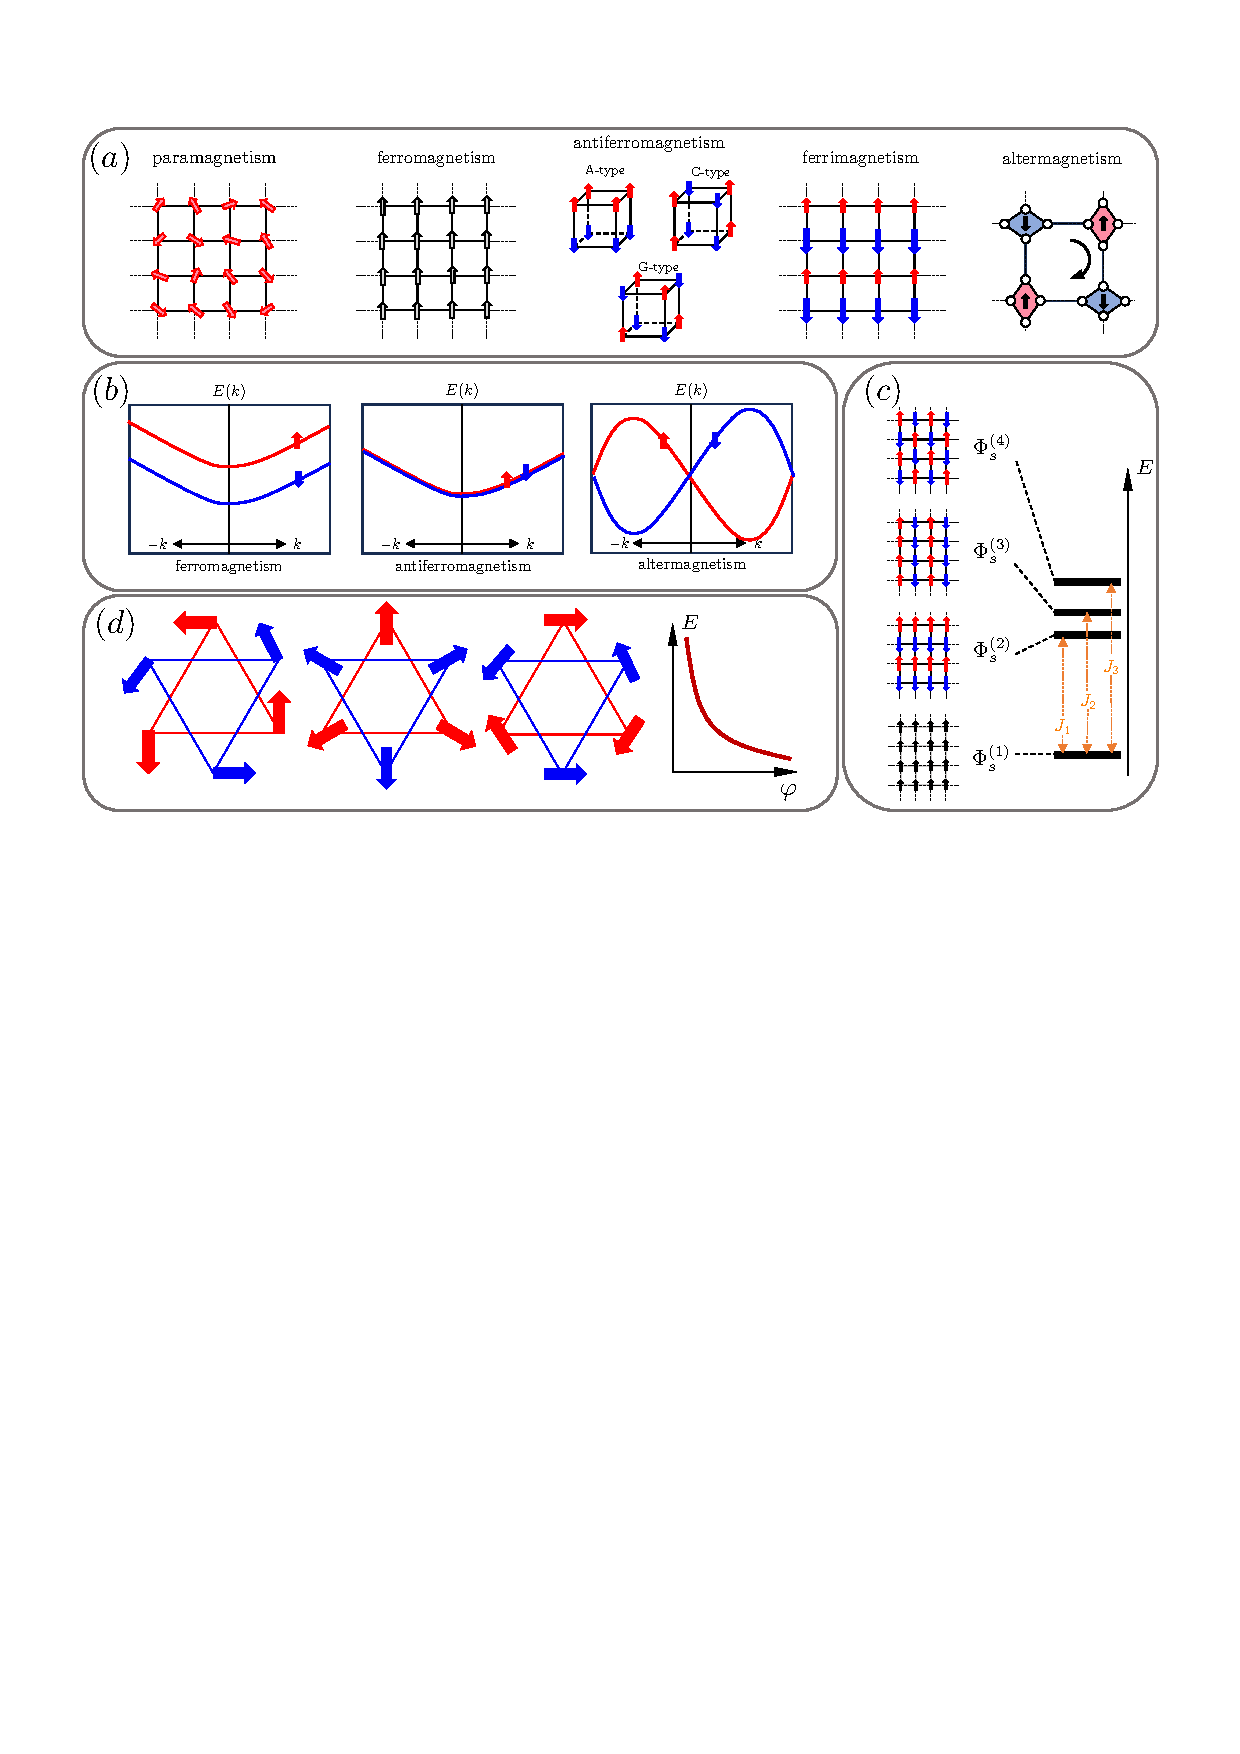
\includegraphics[width=\linewidth]{mangetic_landscape.pdf}
    \caption{Landscape of magnetic states in solids. (a) Five types of commonly known colinear magnetic states, illustrating the spatial spin configurations in a simple square/cubic lattice. (b) Reciprocal-space (band-structural) interpretations of ferromagnetism, antiferromagnetism and altermagnetism in solids. (c) The energy landscape of different magnetic states in a given solid, in which the energetic differences between spin configurations can be used to infer the exchange coupling constants $J$. (d) Illustration of non-colinear spin configurations in a hexagonal lattice, in which the total energy of the system now varies as a function of the canting angle between the two neighbouring interacting spins. }
    \label{fig:mangetic_landscape}
\end{figure}

As such, to better understand the role of modern DFT in studying the magnetic properties of materials, it is important to first briefly account for the common types of magnetic states in materials. Broadly speaking, there are two categories of magnetic states in condensed matters, which, as to be discussed later, also leads to two different approaches on how spin densities are treated in DFT: (a) 
\textit{colinear magnetism} [\cref{fig:mangetic_landscape}(a)], in which the spin moments are all aligned along a fixed global axis (typically the $z$-axis), and (b) \textit{non-colinear magnetism} [\cref{fig:mangetic_landscape}(d)], in which spins are not restricted to be aligned with a given axis, but still adopt a distinct spiral/helical texture. 


In the case of colinear magnetism, three different types of spin configurations are most well known from basic solid state physics:\cite{kittel2018introduction} (i) \textit{Ferromagnetism}, in which all neighbouring spins are parallel aligned with each other, giving rise to a net magnetic moment in the material. (ii) \textit{Antiferromagnetism}, in which the system exhibits no net magnetisation, since the total magnetic moment from the up-spin sublattice is perfectly compensated by that from the down-spin sublattice. Furthermore, depending on the relative spatial relationship between the up- and down-spin sublattices, the antiferromagnetic state can be further categorised as A-, C- or G-type, which can be energetically distinguished using computational techniques.\cite{horton2019high,chang2021electronic,kassimi2023electronic} (iii) \textit{Ferrimagnetism}, which is similar to antiferromagnetism except that the oppositely aligned magnetic moments are of different magnitudes, leading to an overall net non-zero magnetisation in the material. In  these three types of colinear magnetism, the spin-spin interactions can all be described by the Heisenberg exchange Hamiltonian $\hat{\mathcal{H}}=\sum_{ij}J_{ij}\bm{s}_i\cdot\bm{s}_j$. In terms of the electronic band structure theory [\cref{sect:band_structure} and \cref{fig:mangetic_landscape}(b)], ferromagnetic materials are typically characterised by non-degenerate spin-up and spin-down dispersion curves in the reciprocal space, whereas for antiferromangetic materials, the spin-up and spin-down energy bands are degenerated across the entire reciprocal space. Finally, (iv) \textit{altermagnetism} has recently attracted\cite{vsmejkal2022beyond,fender2025altermagnetism} many research interests as an unconventional colinear magnetism, although the phenomenon was first generally identified some thirty years ago.\cite{solovyev1997magneto} It typically appears in non-centrosymmetric crystals whereby two ferromagnetic sublattices are structurally related to each other by a rotational operation and become antiferromagnetically coupled to each other, hence the materials appear to be antiferromagnetic overall. In terms of the band structure theory, altermagnet manifests itself with the reversal of band energy ordering upon the inversion of the linear momentum, \textit{i.e.} $E(\bm{k},\bm{s}_i)=-E(-\bm{k},\bm{s}_i)$ [\cref{fig:mangetic_landscape}(b)], which necessitates the introduction of a linear-momentum-dependent exchange term in the Heisenberg Hamiltonian to describe altermagnetism, \textit{i.e.}, $\hat{\mathcal{H}}=\sum_{ij}J_{ij}(\bm{k})\bm{s}_i\cdot\bm{s}_j$.

Without considering the contributions from crystal structures, spin-orbit coupling in heavy elements is regarded as one of the prominent sources of non-colinear magnetism in materials. The spin-orbit coupling is described by the Hamiltonian $\hat{\mathcal{H}}=\lambda(\bm{L}\cdot\bm{s})$, which couples the orbital angular momentum $\bm{L}$ with the spin magnetic moment $\bm{s}$. This makes the spin orientation become tied to the direction of electronic motion around the nucleus, resulting in spin canting relative to each other. Non-linear magnetic states are also observed in 120$^\circ$-oriented triangular lattices,\cite{sakuma2002magnetic,wang2008spin,yin2022topological} which favour the spin configurations in which neighbouring spins pointing 120$^\circ$ away from each other and is an example of non-colinear magnetism that is induced by geometric frustration. As shown in \cref{fig:mangetic_landscape}(d), the energy of this system becomes a function of the canting angle between two neighbouring spin,\cite{baumsteiger2025exploring} which can also be physically described by the Heisenberg exchange Hamiltonian. Finally, the Dzyaloshinskii-Moriya\cite{dzyaloshinsky1958thermodynamic,moriya1960anisotropic} interactions, which is predominant in systems with strong spin-orbit interaction that is coupled with crystal structures lacking the inversion symmetry. The Dzyaloshinskii-Moriya interaction can be described by the Hamiltonian $\hat{\mathcal{H}}=\sum_{ij}\bm{D}_{ij}\cdot(\bm{s}_i\times\bm{s}_j)$, in which the cross-product antisymmetrised the spin-spin interactions under the exchange of $i$ and $j$, where as $\bm{D}_{ij}$ is the so-called Dzyaloshinskii-Moriya vector whose magnitude and direction are determined by the crystal symmetry and the strength of spin–orbit coupling. The outcome of this special type of spin interaction is that it favours the configuration of chiral spin canting, in which spins tend to twist around a given axis with a fixed chirality.   
 
We note that, strictly speaking, paramagnetism, in which spins across lattice sites are randomly aligned with respect to each other, is strictly speaking, a non-colinear magnetic state. It is the magnetic state that occurs above the magnetic phase transition temperatures that both colinear and non-colinear magnetic alignments become thermally randomised. It is only grouped into \cref{fig:mangetic_landscape}(a) because the concept of paramagnetism is traditionally introduced in the solid-state textbooks along with the colinear magnetism.

Building on the knowledge of these different spin configurations that can occur in solids, it enables us to construct a physically sensible workflow that combines with DFT to calculate and compare the relative energetic stabilities of different magnetic states in a material. This allows us to identify the most favourable ground state and to probe how competing interactions shape the magnetic landscape. In particular, the energy difference between the ground and next metastable magnetic state can be used to compute the magnitude of the exchange coupling constant [\cref{fig:mangetic_landscape}(c) as illustrated for the case of colinear magnetism], which can be further applied to estimate macroscopic properties, such as magnetic transition temperatures. For the case of non-colinear magnetisms, such as those occurring in the frustrated triangular lattices [\cref{fig:mangetic_landscape}], one would need to perform additional sampling of the energy landscape by varying the canting angle between a pair of neighbouring spins $\bm{s}_i$ and $\bm{s}_j$ while keeping the spin orientations on the other lattice sites fixed.\cite{baumsteiger2025exploring}  

Finally, before the end of this section, we shall briefly discuss the theoretical foundations of DFT to account for the spin degree of freedom in modelling the physical properties of materials. For colinear magnetism,\cite{von1972local,gunnarsson1976exchange} extending the KS formalism to account for spin polarisation is straightforward, in which the total electron density is simply the sum of the spin-up and spin-down densities over all the occupied states, \emph{i.e.} $\rho(\bm{r})=\sum\limits_{i=\mbox{\scriptsize{occ.}}}\sum\limits_{\sigma=\uparrow,\downarrow}\left\vert \varphi_{i,\sigma}(\bm{r}) \right\vert^2$. Differentiating the contributions from spin-up and spin-down electron densities to the total system energy can be achieved by making the KS potential become explicitly spin-dependent as $E_{xc}^{\sigma}(\rho_\sigma (\bm{r}))$, such that electrons with opposite spin orientations shall experience different spin-dependent potentials. In LDA, for instance, this can be achieved with the following functional for the exchange energy:
\begin{equation*}
    E_{x}[\rho_{\uparrow}(\bm{r}),\rho_{\downarrow}(\bm{r})]=-C_{x}\int\left(\rho_{\uparrow}(\bm{r})^{\frac{4}{3}}+\rho_{\downarrow}(\bm{r})^{\frac{4}{3}}\right) \mbox{d}\bm{r},
\end{equation*}
or equivalently expressed with the spin polarisation factor $\zeta=(\rho_{\uparrow}-\rho_{\downarrow})/\rho$, with $\rho=\rho_{\uparrow}+\rho_{\downarrow}$ as:
\begin{equation*}
    E_{x}(\rho,\zeta)=E_{x}(\rho,0)\frac{(1+\zeta)^{\frac{4}{3}}+(1-\zeta)^{\frac{4}{3}}}{2}.
\end{equation*}
On the other hand, to treat non-colinear magnetic states,\cite{kubler1988density,kurz2004ab,peralta2007noncollinear} one can no longer treat the electron density as a scalar quantity, but the spin-density matrix, which is constructed as the Kronecker product between two two-component spin-density vectors as: 
\begin{equation}
    \label{eq:density_matrix}
    \bm{\rho}(\bm{r})=\sum_{n\bm{k}}f_{n\bm{k}}\left(\varphi^{*}_{n\bm{k},\uparrow}(\bm{r}),\varphi^{*}_{n\bm{k},\downarrow}(\bm{r})\right)\left(\begin{array}{c}
        \varphi_{n\bm{k},\uparrow}(\bm{r})  \\
         \varphi_{n\bm{k},\downarrow}(\bm{r})
    \end{array}\right)=\left(\begin{array}{cc}
      \rho_{\uparrow\uparrow}(\bm{r})   &  \rho_{\uparrow\downarrow}(\bm{r})\\
      \rho_{\downarrow\uparrow}(\bm{r})   & \rho_{\downarrow\downarrow}(\bm{r})
    \end{array} \right),
\end{equation}
in which the off-diagonal elements $\rho_{\uparrow\downarrow}(\bm{r})$ and $\rho_{\downarrow\uparrow}(\bm{r})$ can map the electron densities to the magnetisations along the $x$ and $y$-directions $(m_x,m_y)$ in addition to the $z$-component $m_z$. This is made obvious by rewriting \cref{eq:density_matrix} in the following form
\begin{equation}
    \rho(\bm{r})=\frac{1}{2}\bigg(\rho(\bm{r})\bm{I}+\bm{m}(\bm{r})\cdot\vec{\sigma})\bigg),
\end{equation}
in which $\bm{m}(\bm{r})=(m_x,m_y,m_z)$ and $\vec{\sigma}$ is the vector of Pauli spin matricies. This thus concludes our short account for studying the magnetic properties of materials with computational approaches.

